% Point to the main file
\documentclass[../../Main.tex]{subfiles}

% ========== Start the document ==========
\begin{document}

\section{Section 2.3 - Functions}

\begin{definition}
    Let $\mathset{A}$ and $\mathset{B}$ be sets

    A \yellowbox{relation} from $\mathset{A}$ to $\mathset{B}$ is a subset of $\mathset{A} \times \mathset{B}$
\end{definition}

\begin{example}
    Let $\mathset{A} = \{ 1, 4, 9 \}$ and $\mathset{B} = \{ \pm 1, \pm 2, \pm 3 \}$

    \begin{enumerate}
        \item $| A \times B | = 3 \cdot 6 = 18 $
        \item Let $R$ be the relation from $A$ to $B$ defined by
        
        $$R = \{ (a, b) \mid a \in A, b \in B, a = b^2 \}$$

        $R = \{ (1, 1), (1, -1), (4, 2), (4, -2), (9, 3), (9, -3) \}$
    \end{enumerate}

\end{example}

\begin{note}
    $R$ is a relation but \underline{not} a function
\end{note}

Why?

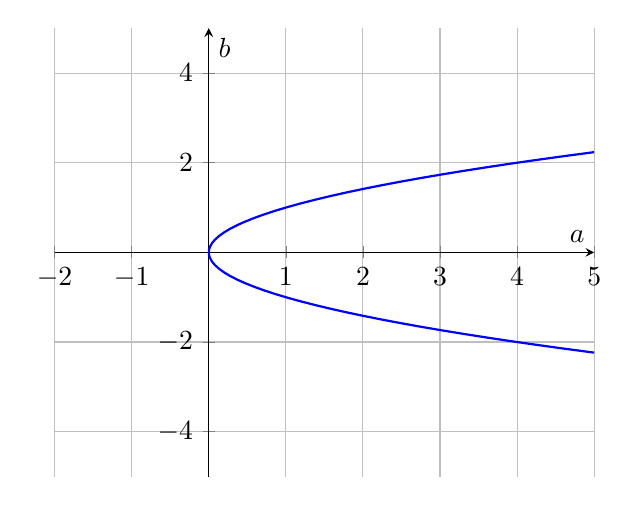
\begin{tikzpicture}
    \begin{axis}[
        axis lines=middle,
        xmin=-2, xmax=5,
        ymin=-5, ymax=5,
        xlabel=$a$, ylabel=$b$,
        grid=both
    ]
        % Plotting a line
        \addplot[
            domain=-4:4, 
            blue, 
            thick,
            samples=100,
            variable=\t
        ] ({t^2}, {t});
        % \addlegendentry{Data B}
        % Marking points
        % \addplot[only marks, mark=*, red] coordinates {(1,0) (3,2)};
        % \addlegendentry{Data A}
        % \node[anchor=west] at (axis cs:3,2) {A(3,2)};
    \end{axis}
\end{tikzpicture}

This graph of the relation fails the vertical line test, hence it is not a function

There exists an element of $A$ that corresponds to more than one element of $B$

\begin{tablewithheader}
{|c|c|}
{a & b}
1 & -1 \\
1 & 1 \\
4 & -2 \\
4 & 2 \\
9 & -3 \\
9 & 3 \\
\end{tablewithheader}

Every function is a relation but not all relations are functions

\begin{definition}[Function]
    Let $A$ and $B$ be sets 

    A \yellowbox{function} $f$ from $A$ to $B$, denoted as

    $$f: A \rightarrow B$$

    is a relation from $A$ to $B$ such that 

    $$\forall a \in A \exists! b \in B, f(a) = b$$

    \begin{center}
        $\exists!$ means "there exists a \textbf{unique}..."
    \end{center}
\end{definition}

\begin{definition}[Domain and Codomain]
    We call the set $A$ the \yellowbox{domain} of $f$ and the set $B$ the \yellowbox{codomain}.

    The \yellowbox{range} or \yellowbox{image} of $f$ is the set 

    $$ \text{Im}(f) = \{ b \in B \mid \exists a \in A, f(a) = b \} $$
\end{definition}

\begin{example}
    Determine if the following are functions

    \begin{enumerate}
        \item $f: \setR \rightarrow \setR, \; f(x) = x^2$
        
        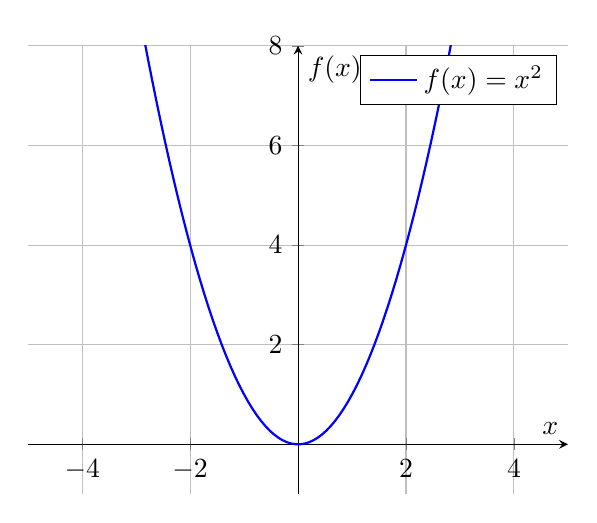
\begin{tikzpicture}
            \begin{axis}[
                axis lines=middle,
                xmin=-5, xmax=5,
                ymin=-1, ymax=8,
                xlabel=$x$, ylabel=$f(x)$,
                grid=both
            ]
                % Plotting a line
                \addplot[
                    domain=-4:4, 
                    blue, 
                    thick,
                    samples=100
                ] {x^2};
                \addlegendentry{$f(x)=x^2$}
                % Marking points
                % \addplot[only marks, mark=*, red] coordinates {(1,0) (3,2)};
                % \addlegendentry{Data A}
                % \node[anchor=west] at (axis cs:3,2) {A(3,2)};
            \end{axis}
        \end{tikzpicture}

        \begin{center}
            Domain: x axis
            \\
            Codomain: y axis
            \\
            $\text{Im}(f) = [0, \infty]$
            \\
            $\therefore$ Yes
        \end{center}

        \item $f: \setR \rightarrow \setR, \; f(x) = \sqrt{x}$
        
        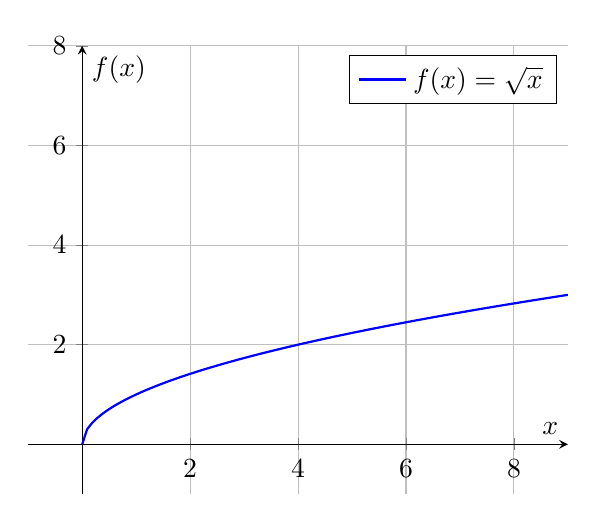
\begin{tikzpicture}
            \begin{axis}[
                axis lines=middle,
                xmin=-1, xmax=9,
                ymin=-1, ymax=8,
                xlabel=$x$, ylabel=$f(x)$,
                grid=both
            ]
                % Plotting a line
                \addplot[
                    domain=0:9, 
                    blue, 
                    thick,
                    samples=100
                ] {sqrt(x)};
                \addlegendentry{$f(x)=\sqrt{x}$}
                % Marking points
                % \addplot[only marks, mark=*, red] coordinates {(1,0) (3,2)};
                % \addlegendentry{Data A}
                % \node[anchor=west] at (axis cs:3,2) {A(3,2)};
            \end{axis}
        \end{tikzpicture}

        \begin{center}
            No since not all inputs are valid
        \end{center}

        \item $f: \setR^+ \rightarrow \setR, \; f(x) = \sqrt{x}$
        
        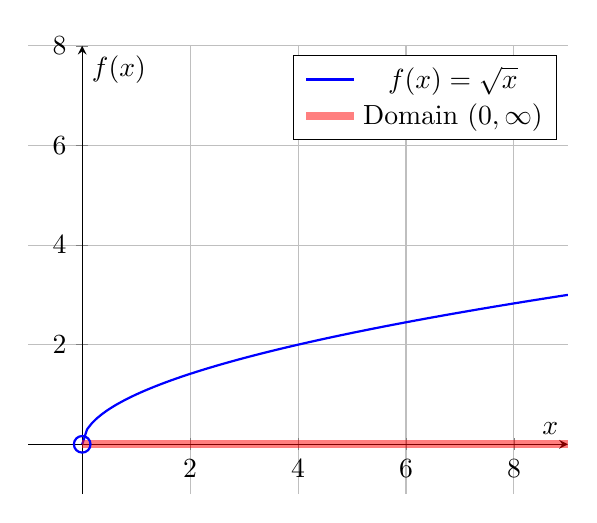
\begin{tikzpicture}
            \begin{axis}[
                axis lines=middle,
                xmin=-1, xmax=9,
                ymin=-1, ymax=8,
                xlabel=$x$, ylabel=$f(x)$,
                grid=both
            ]
                % Plotting a line
                \addplot[
                    domain=0:9, 
                    blue, 
                    thick,
                    samples=100
                ] {sqrt(x)};
                \addlegendentry{$f(x)=\sqrt{x}$}

                % Highlight the x axis
                \draw[line width=3pt, red, opacity=0.5] (axis cs:0,0) -- (axis cs:10,0);

                \addlegendimage{line width=3pt, red, opacity=0.5}
                \addlegendentry{Domain $(0, \infty)$}

                % The "Excluded" Point at (0,0)
                \addplot[
                    only marks,
                    mark=o,          % 'o' for open circle
                    mark size=3pt,   % make it visible
                    thick,           % thickness of the circle border
                    fill=white,      % ensures it masks the axis lines
                    draw=blue       % color of the ring
                ] coordinates {(0,0)};
                % Marking points
                % \addplot[only marks, mark=*, red] coordinates {(1,0) (3,2)};
                % \addlegendentry{Data A}
                % \node[anchor=west] at (axis cs:3,2) {A(3,2)};
            \end{axis}
        \end{tikzpicture}

        $$ \text{Im}(f) = (0, \infty) $$

        Yes since all the inputs have a unique output (the origin is excluded since the domain is $\setR^+$)

        \item $f: \setR \rightarrow \setZ, \; f(x) = \lfloor x \rfloor$ \; (floor function, aka greatest integer function) 

        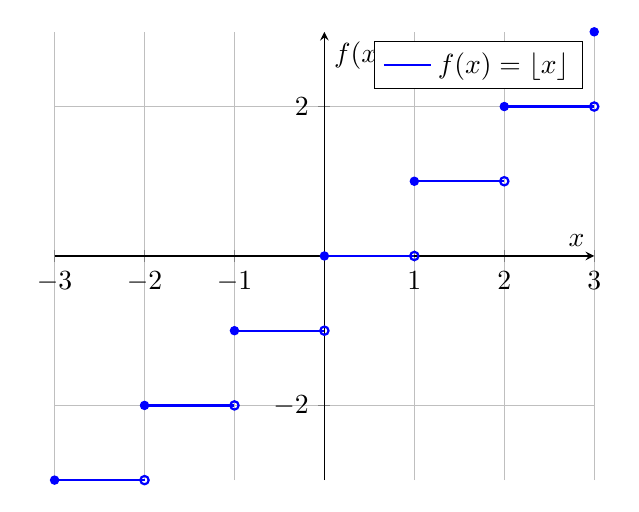
\begin{tikzpicture}
            \begin{axis}[
                axis lines=middle,
                xmin=-3, xmax=3,
                ymin=-3, ymax=3,
                xlabel=$x$, ylabel=$f(x)$,
                grid=both
            ]
                % Plotting a line
                \addplot[
                    blue, 
                    thick, 
                    domain=-3:3, 
                    samples=7, % One sample per integer step
                    jump mark left
                    % const plot
                ] {floor(x)};
                \addlegendentry{$f(x) = \lfloor x \rfloor$}
                % 2. Add Closed Circles (Left end: Included)
                \addplot[
                    only marks, 
                    mark=*, 
                    mark size=1.5pt, 
                    blue
                ] coordinates {(-3,-3) (-2,-2) (-1,-1) (0,0) (1,1) (2,2) (3,3)};

                % 3. Add Open Circles (Right end: Excluded)
                \addplot[
                    only marks, 
                    mark=o, 
                    mark size=1.5pt, 
                    thick, 
                    blue, 
                    fill=white % This hides the grid/axis behind the circle
                ] coordinates {(-2,-3) (-1,-2) (0,-1) (1,0) (2,1) (3,2) (4,3)};
                
                % Marking points
                % \addplot[only marks, mark=*, red] coordinates {(1,0) (3,2)};
                % 
                % \node[anchor=west] at (axis cs:3,2) {A(3,2)};
            \end{axis}
        \end{tikzpicture}

        \begin{tablewithheader}
        { |c|c| }
        { $x$ & $\lfloor x \rfloor$ }
        -1 & -1 \\
        0 & 0 \\
        0.5 & 0 \\
        0.99 & 0 \\
        1.01 & 1 \\
        \end{tablewithheader}

        $$ \text{Im}(f) = \setZ $$

        All of x axis is domain, but only \textbf{integer} parts of y axis is codomain

        \item $f: \setR \rightarrow \setZ, \; f(x) = \lceil x \rceil$ \; (ceiling function, aka least integer function) 

        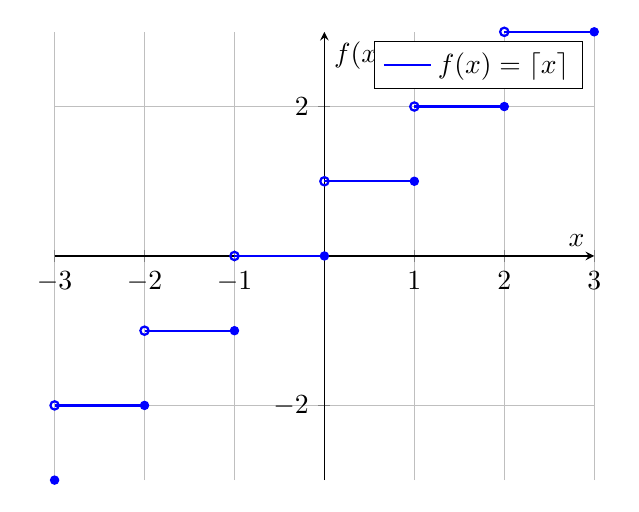
\begin{tikzpicture}
            \begin{axis}[
                axis lines=middle,
                xmin=-3, xmax=3,
                ymin=-3, ymax=3,
                xlabel=$x$, ylabel=$f(x)$,
                grid=both
            ]
                % Plotting a line
                \addplot[
                    blue, 
                    thick, 
                    domain=-3:3, 
                    samples=7, % One sample per integer step
                    jump mark right
                    % const plot
                ] {ceil(x)};
                \addlegendentry{$f(x) = \lceil x \rceil$}

                % 2. Add Open Circles (Left end: Excluded)
                \addplot[
                    only marks, 
                    mark=*, 
                    mark size=1.5pt, 
                    blue
                ] coordinates {(-3,-3) (-2,-2) (-1,-1) (0,0) (1,1) (2,2) (3,3)};

                % % 3. Add Closed Circles (Right end: Included)
                \addplot[
                    only marks, 
                    mark=o, 
                    mark size=1.5pt, 
                    thick, 
                    blue, 
                    fill=white % This hides the grid/axis behind the circle
                ] coordinates {(-4,-3) (-3,-2) (-2,-1) (-1,0) (0,1) (1,2) (2,3)};
                
                % Marking points
                % \addplot[only marks, mark=*, red] coordinates {(1,0) (3,2)};
                % 
                % \node[anchor=west] at (axis cs:3,2) {A(3,2)};
            \end{axis}
        \end{tikzpicture}

        \begin{tablewithheader}
        { |c|c| }
        { $x$ & $\lfloor x \rfloor$ }
        -1 & -1 \\
        0 & 0 \\
        0.5 & 1 \\
        0.99 & 1 \\
        1.01 & 2 \\
        \end{tablewithheader}

        $$ \text{Im}(f) = \setZ $$

        All of x axis is domain, but only \textbf{integer} parts of y axis is codomain

    \end{enumerate}

\end{example}

\begin{definition}[Surjective]
    Let $f: A \rightarrow B$ be a function in the set $A$ and $B$

    We say $f$ is \yellowbox{onto} or \yellowbox{surjective} if

    \begin{center}
        $ \text{Im}(f) = B $

        or

        $ \forall b \in B \exists a \in A, \; f(a) = b $

        or

        All of codomain is covered by the function
    \end{center}

\end{definition}

\begin{definition}[Injective]
    We say $f$ is \yellowbox{one to one} or \yellowbox{injective} if 

    $$ \forall b \in B, \text{ the equation } f(a) = b \text{ has at most on solution}$$

    Another way of thinking of this is:

    \begin{center}
        Injective if it passes the horizontal line test

        or

        there is a unique $b$ for all $a$
        
        or

        no two inputs have the same output

        or

        $f(a) = f(b) \implies a = b$
    \end{center}
\end{definition}

\begin{definition}[Bijective]
    If $f$ is both \textbf{surjective} and \textbf{injective}, then we say $f$ is \yellowbox{bijective}
\end{definition}

\begin{example}
    Determine if the following functions are injective, surject, and / or bijective

    \begin{enumerate}
        \item $f: \setR \rightarrow \setR, \; f(x) = e^x$
        
        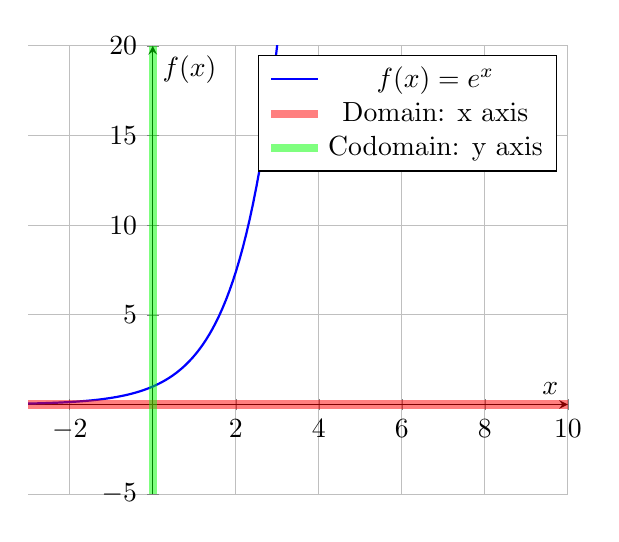
\begin{tikzpicture}
            \begin{axis}[
                axis lines=middle,
                xmin=-3, xmax=10,
                ymin=-5, ymax=20,
                xlabel=$x$, ylabel=$f(x)$,
                grid=both
            ]
                % Plotting a line
                \addplot[
                    domain=-3:5, 
                    blue, 
                    thick,
                    samples=100
                ] {e^x};
                \addlegendentry{$f(x)=e^x$}

                % Highlight the x axis
                \draw[line width=3pt, red, opacity=0.5] (axis cs:-3,0) -- (axis cs:10,0);
                \addlegendimage{line width=3pt, red, opacity=0.5}
                \addlegendentry{Domain: x axis}

                % Highlight the y axis
                \draw[line width=3pt, green, opacity=0.5] (axis cs:0,-5) -- (axis cs:0,20);
                \addlegendimage{line width=3pt, green, opacity=0.5}
                \addlegendentry{Codomain: y axis}

                % The "Excluded" Point at (0,0)
                % \addplot[
                %     only marks,
                %     mark=o,          % 'o' for open circle
                %     mark size=3pt,   % make it visible
                %     thick,           % thickness of the circle border
                %     fill=white,      % ensures it masks the axis lines
                %     draw=blue       % color of the ring
                % ] coordinates {(0,0)};
                % Marking points
                % \addplot[only marks, mark=*, red] coordinates {(1,0) (3,2)};
                % \addlegendentry{Data A}
                % \node[anchor=west] at (axis cs:3,2) {A(3,2)};
            \end{axis}
        \end{tikzpicture}

        \begin{center}
            \greentext{Injective} since all x values have a valid output

            \redtext{Not surjective} since not all values on the y axis have a corresponding input value

            \redtext{Not bijective} since it's not surjective
        \end{center}

        \item $f: \setR \rightarrow \setR^+, \; f(x) = e^x$
        
        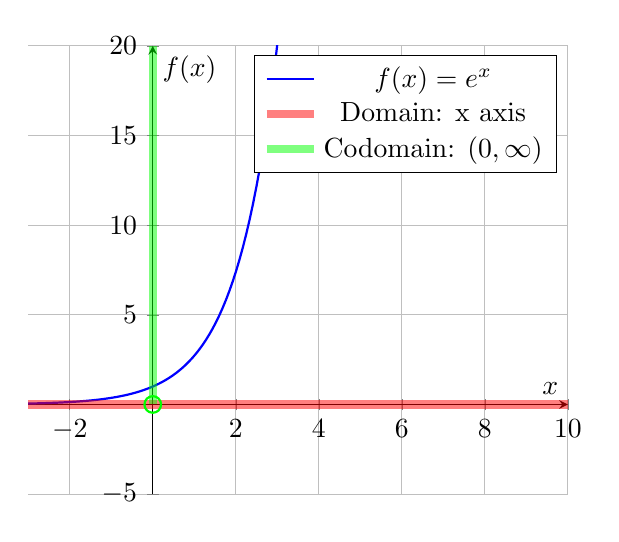
\begin{tikzpicture}
            \begin{axis}[
                axis lines=middle,
                xmin=-3, xmax=10,
                ymin=-5, ymax=20,
                xlabel=$x$, ylabel=$f(x)$,
                grid=both
            ]
                % Plotting a line
                \addplot[
                    domain=-3:5, 
                    blue, 
                    thick,
                    samples=100
                ] {e^x};
                \addlegendentry{$f(x)=e^x$}

                % Highlight the x axis
                \draw[line width=3pt, red, opacity=0.5] (axis cs:-3,0) -- (axis cs:10,0);
                \addlegendimage{line width=3pt, red, opacity=0.5}
                \addlegendentry{Domain: x axis}

                % Highlight the y axis
                \draw[line width=3pt, green, opacity=0.5] (axis cs:0,0) -- (axis cs:0,20);
                \addlegendimage{line width=3pt, green, opacity=0.5}
                \addlegendentry{Codomain: $(0, \infty)$}

                % The "Excluded" Point at (0,0)
                \addplot[
                    only marks,
                    mark=o,          % 'o' for open circle
                    mark size=3pt,   % make it visible
                    thick,           % thickness of the circle border
                    fill=white,      % ensures it masks the axis lines
                    draw=green       % color of the ring
                ] coordinates {(0,0)};
                % Marking points
                % \addplot[only marks, mark=*, red] coordinates {(1,0) (3,2)};
                % \addlegendentry{Data A}
                % \node[anchor=west] at (axis cs:3,2) {A(3,2)};
            \end{axis}
        \end{tikzpicture}

        \begin{center}
            \greentext{Injective} since all x values have a valid output

            \greentext{Surjective} since all values on the y axis have a corresponding input value

            \greentext{Bijective} since it's both surjective and injective
        \end{center} 

    \end{enumerate}

    There's more examples, write them down when you get the chance

\end{example}

\begin{definition}[Composition]
    Given the functions $f: B \rightarrow C$ and $g: A \rightarrow B$

    Where $A, B, C$ are  sets, then we define

    $$ f \circ g: A \rightarrow B \; \text{ by}$$ 

    $$ (f \circ g)(a) = f( g(a) ) $$

    called the \yellowbox{composition} of $f$ and $g$

\end{definition}

\includegraphics[width=12cm]{Composition.png}

\begin{example}[Examples of Compositions]
    
    Let $f(x) = x - 3, \; g(x) = x^3 + 9x^2 + 27x + 27 = (x + 3)^3 $

    Compute the following

    \begin{enumerate}
        \item $(f \circ g)(x)$
        
        \begin{align*}
            (f \circ g)(x) &= f(g(x)) \\
            &= (x^3 + 9x^2 + 27x + 27) - 3 \\
            &= x^3 + 9x^2 + 27x + 24 \\
        \end{align*}

        \item $(g \circ f)(x)$
        
        \begin{align*}
            (g \circ f)(x) &= g(f(x)) \\
            &= (x - 3)^3 + 9(x-3)^2 + 27(x-3) + 27 \\
            &= \left[ (x-3) +3 \right]^3 \\
            &= x^3 \\
        \end{align*}
    \end{enumerate}

\end{example}

% ========== End the document ==========
\end{document}